% !TeX root = ../main.tex

\chapter{图表,代码和其他环境}

\section{浮动体位置参数}
\begin{description}
  \item[h] 将浮动体放置在当前位置,如果当前位置无法容纳,则放置在页面顶部。
  \item[t] 将浮动体放置在页面顶部。
  \item[b] 将浮动体放置在页面底部。
  \item[p] 将浮动体放置在单独的一页中。
  \item[H] 强制将浮动体放置在当前位置,而不管当前位置是否能容纳。
\end{description}
此外,还可以使用叹号!来增加强制性,例如\verb|[!t]|表示强制将浮动体放置在页面顶部。一般用\verb|[ht]|或\verb|[htbp]|。

\section{图片}

\subsection{插入单个图片}
\begin{figure}[ht]
    \centering
    
\includegraphics[width=0.5\linewidth]{264498559_cover.png}
    \caption{Enter Caption}
    \label{fig:enter-label}
\end{figure}

\begin{figure}[ht]
  \centering
  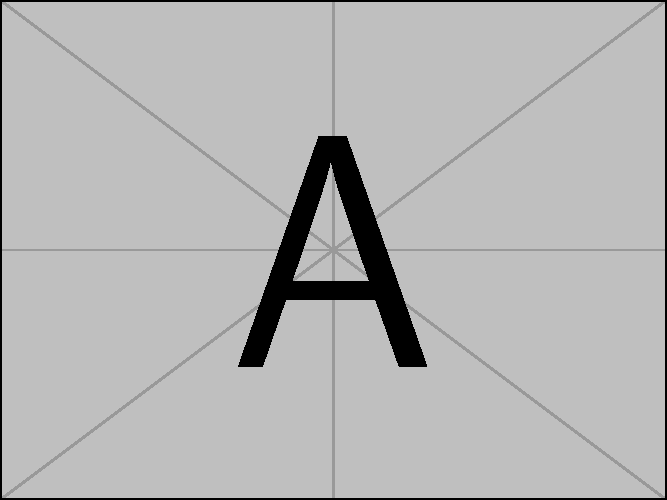
\includegraphics[width=0.3\linewidth]{example-image-a.pdf}
  \caption{示例图片标题}
  \label{fig:example}
\end{figure}

\subsection{插入偏左或偏右的图片}

\begin{wrapfigure}
  [7]{r}{80mm}  % 竖列7行,靠右排,宽度80mm
  \centering
  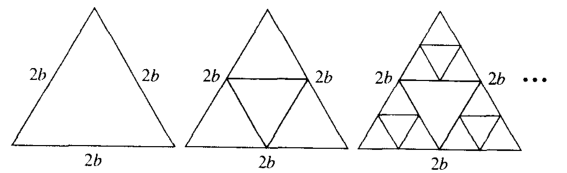
\includegraphics[width=80mm]{jishu-lianxi.png}
  \caption{一个三角形图形序列}
  \label{fig:triangle}
\end{wrapfigure}
如图~\ref{fig:triangle}~所示,有一个边长为$2b$的正三角形,从中挖去一个倒放的正三角形,重复这个步骤,被挖去的面积之和形成一个无穷级数。\\
(a)求这个无穷级数;\\
(b)求这个级数和;\\
(c)是否原来三角形中的每个点都被挖去了?解释为什么。
\begin{lstlisting}[language=tex]
\begin{wrapfigure}
  [行数]{位置}{超出长度}{宽度}<图形>  % 注意,行数两边是方括号,不是花括号
\end{wrapfigure}
\end{lstlisting}

\subsection{插入两个并排的图片}
\begin{figure}[H]
  \centering
  \begin{minipage}{0.48\textwidth}
  \centering
  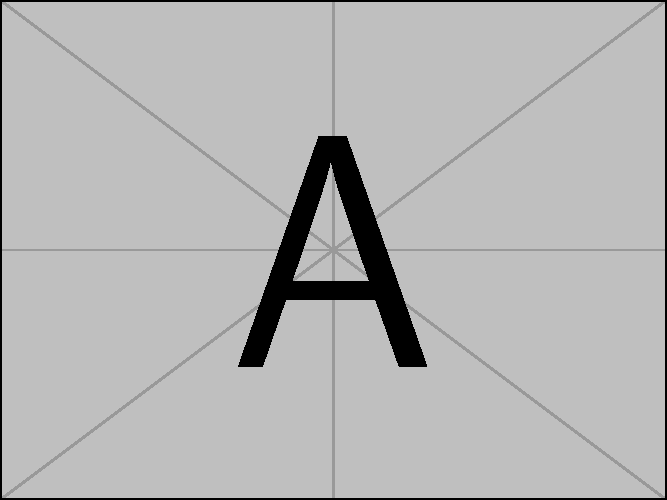
\includegraphics[width=50mm]{example-image-a.pdf}
  \caption{标题1}
  \end{minipage}
  \begin{minipage}{0.48\textwidth}
  \centering
  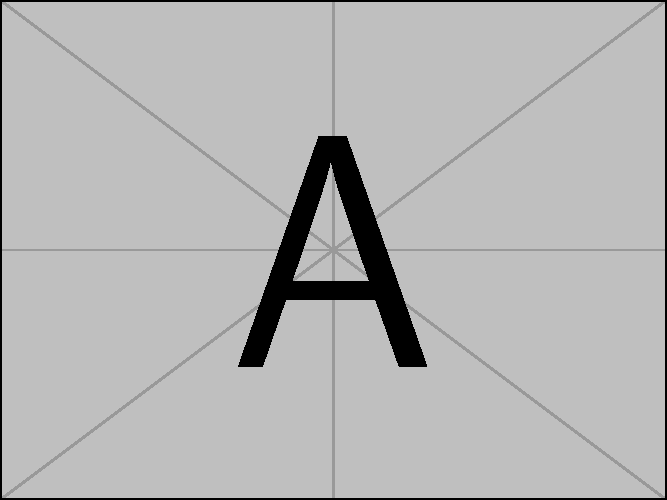
\includegraphics[width=50mm]{example-image-a.pdf}
  \caption{标题2}
  \end{minipage}
\end{figure}

\subsection{解决图片/表格过宽的问题}

\begin{lstlisting}[language=tex]
% \usepackge{graphicx}
\resizebox{\textwidth}{!}{
    %图片/表格内容
}
\end{lstlisting}


\section{表格}

三线表,如表~\ref{tab:three-line}。

\begin{table}[htbp]
  \centering
  \caption{三线表示例}
  \begin{tabular}{ll}
    \toprule
    文件名          & 描述       \\
    \midrule
    thuthesis.dtx   & 模板的源文件,包括文档和注释  \\
    thuthesis.cls   & 模板文件  \\
    thuthesis-*.bst & BibTeX 参考文献表样式文件  \\
    \bottomrule
  \end{tabular}
  \label{tab:three-line}
\end{table}

表格如果有附注,尤其是需要在表格中进行标注时,可以使用\verb|threeparttable|宏包。

\begin{table}[ht]
  \centering
  \begin{threeparttable}[c]
    \caption{带附注的表格示例}
    \label{tab:three-part-table}
    \begin{tabular}{ll}
      \toprule
      文件名                 & 描述                         \\
      \midrule
      thuthesis.dtx\tnote{a} & 模板的源文件,包括文档和注释 \\
      thuthesis.cls\tnote{b} & 模板文件                     \\
      thuthesis-*.bst        & BibTeX 参考文献表样式文件    \\
      \bottomrule
    \end{tabular}
    \begin{tablenotes}
      \item [a] 可以通过 xelatex 编译生成模板的使用说明文档。
      \item [b] 更新模板。
    \end{tablenotes}
  \end{threeparttable}
\end{table}

如某个表需要转页接排,可以使用\verb|longtable| 宏包,需要在随后的各页上重复表的编号。
编号后跟表题(可省略)和“(续)”,置于表上方。续表均应重复表头。

\begin{longtable}{cccc}
    \caption{跨页长表格的表题}
    \label{tab:longtable} \\
    \toprule
    表头 1 & 表头 2 & 表头 3 & 表头 4 \\
    \midrule
  \endfirsthead
    \caption*{续表~\thetable\quad 跨页长表格的表题} \\
    \toprule
    表头 1 & 表头 2 & 表头 3 & 表头 4 \\
    \midrule
  \endhead
    \bottomrule
  \endfoot
  Row 1  & & & \\
  Row 2  & & & \\
  Row 3  & & & \\
  Row 4  & & & \\
  Row 5  & & & \\
  Row 6  & & & \\
  Row 7  & & & \\
  Row 8  & & & \\
  Row 9  & & & \\
  Row 10 & & & \\
  Row 11 & & & \\
  Row 12 & & & \\
  Row 13 & & & \\
  Row 14 & & & \\
  Row 15 & & & \\
  Row 16 & & & \\
  Row 17 & & & \\
  Row 18 & & & \\
  Row 19 & & & \\
  Row 20 & & & \\
\end{longtable}



\section{算法}

\renewcommand{\algorithmicrequire}{\textbf{输入:}\unskip}
\renewcommand{\algorithmicensure}{\textbf{输出:}\unskip}

\begin{algorithm}
  \caption{Calculate $y = x^n$}
  \label{alg1}
  \small
  \begin{algorithmic}
    \REQUIRE $n \geq 0$
    \ENSURE $y = x^n$

    \STATE $y \leftarrow 1$
    \STATE $X \leftarrow x$
    \STATE $N \leftarrow n$

    \WHILE{$N \neq 0$}
      \IF{$N$ is even}
        \STATE $X \leftarrow X \times X$
        \STATE $N \leftarrow N / 2$
      \ELSE[$N$ is odd]
        \STATE $y \leftarrow y \times X$
        \STATE $N \leftarrow N - 1$
      \ENDIF
    \ENDWHILE
  \end{algorithmic}
\end{algorithm}


\section{代码}

\begin{lstlisting}[language=c]
#include<stdio.h>

int main(){
  printf("Hello!\n");  // 输出你好
  return 0;
}
\end{lstlisting}

\begin{lstlisting}[language=python]
import random
import collections
Card = collections.namedtuple('Card', ['rank', 'suit'])
# 一个叫做 FrenchDesk 的类。a class named FrenchDesk.
class FrenchDesk:
    ranks = [str(n) for n in range(2, 11)] + list('JQKA')
    suits = 'spades diamonds clubs hearts'.split()
    
    def __init__(self):
        self._cards = [Card(rank, suit) for rank in self.ranks for suit in self.suits]
        
    def __len__(self):
        return len(self._cards)
        
    def __getitem__(self, position):
        return self._cards[position]
desk = FrenchDesk()
\end{lstlisting}


\section{列表}

\subsection{无序列表}

\begin{itemize}
  \item 文本1
  \item 文本2
\end{itemize}

\subsection{编号列表}

\begin{enumerate}
  \item 文本1
  \item 文本2 
\end{enumerate}

\subsection{描述列表}

\begin{description}
  \item[First] 文本1
  \item[Second] 文本2
\end{description}

